% Activate the following line by filling in the right side. If for example the name of the root file is Main.tex, write
% "...root = Main.tex" if the chapter file is in the same directory, and "...root = ../Main.tex" if the chapter is in a subdirectory.
 
%!TEX root =  ../Thesis.tex

\chapter[Reconstruction and Performance]{Event Reconstruction and Performance}



%http://arxiv.org/pdf/0802.1189.pdf
%http://iopscience.iop.org/1126-6708/2008/04/063/pdf/1126-6708_2008_04_063.pdf
\section{Jet Reconstruction}
Jet reconstruction is the process of assembling calorimeter deposits together into a physics object, called a jet, that ideally will do a good job of representing the characteristics ($p_T$, energy, flavor) of the quark or gluon that originated the jet.  There are a number of clustering algorithms for assembling the calorimeter cells, and post-processing steps for improving the performance of jets in analyses--pileup subtraction, energy calibrations, grooming and trimming, to name a few.  

The default jet clustering algorithm in ATLAS is the anti-$k_t$ algorithm with a distance parameter of 0.4.  Roughly summarized, this algorithm starts with a calorimeter cell that has an energy deposit at least $4\sigma$ higher in energy than the ambient and pileup noise, and then the surrounding cells with at least $2\sigma$ more energy than noise are grouped into the jet in a way that prioritizes high energy over close proximity.  The result is that soft deposits get clustered in with hard deposits, rather than clustering amongst themselves.  The distance parameter of 0.4 is a cutoff as to how far away from the seed to look for additional deposits.  

A critical feature of this algorithm, or any jet algorithm, is that it be infrared and collinear safe.  That means when additional `ghost' particles with infinitesimally small energy or infinitesimally close radius are added to the area in and around the jet, the properties of the resulting jet do not change.  Critically, the anti-$k_t$ algorithm is both infrared and collinear safe.






%https://twiki.cern.ch/twiki/bin/view/AtlasPublic/LuminosityPublicResults#Data_Taking_Efficiency_and_Pileu
%http://cds.cern.ch/record/1459529
%https://cds.cern.ch/record/1435196/files/ATLAS-CONF-2012-042.pdf
%https://cds.cern.ch/record/1522015/files/ATL-COM-PHYS-2013-251.pdf

\section{Pileup Calibration and Removal}
\label{sec:pileup}
All the detector subsystems are affected by the presence of pileup, which are collisions other than the hard scatter collision in a given bunch crossing.  As the LHC delivers higher luminosity for a given number of proton bunches, the luminosity increase comes at the price of many interactions per bunch crossing, and these softer interactions create extra activity in the detector that tends to make events noisier and more challenging to reconstruct accurately.  In 2012, the mean number of interactions per crossing ranged from about 10 up to about 40.  

The inner detector and tracking provide an important tool for understanding in-time pileup.  In-time pileup is additional soft interactions in the same bunch crossing as the hard scatter.  The tracking allows primary vertex reconstruction with a resolution fine enough in z$_0$, for the pixels typically $z_0\sin\theta$, to resolve separate primary vertices from each other.   The calorimeters cannot resolve individual primary vertices with such precision, though, so a constant struggle in ATLAS is to measure the calorimeter deposits that come from pileup interactions, and where possible to apply corrections that subtract away pileup contributions to jets from the hard scatter.  On average, each additional pileup vertex in an event adds 370(850) MeV to the p$_T$ of a jet reconstructed with the Anti-kT algorithm with R=0.4(0.6).

In addition to in-time pileup, the calorimeters are prone to out-of-time pileup where the signal in a given in event can be affected by the energy flow of previous collisions because of the calorimeter readout signal shapes.  Out-of-time pileup has the effect of adding an average of 60(210) MeV to central jets, and decreasing the forward jets by 350(470) MeV.  

Corrections for both in-time and out-of-time pileup are derived using Monte Carlo simulation of pileup events overlaid on MC simulation of hard scatter events.  The corrections are then validated in data, in a number of different ways.  Two prominent methods are validation in prompt photon events, which produce a $\gamma$+jet signature where the photon is not affected by pileup.  Then the ratio of the p$_T$ of the two objects can be compared to the p$_T$ ratio found in MC, $p^{jet}_T/p^{ref}_T = p^{jet}_T/p^{\gamma}_T$.


\begin{figure}
	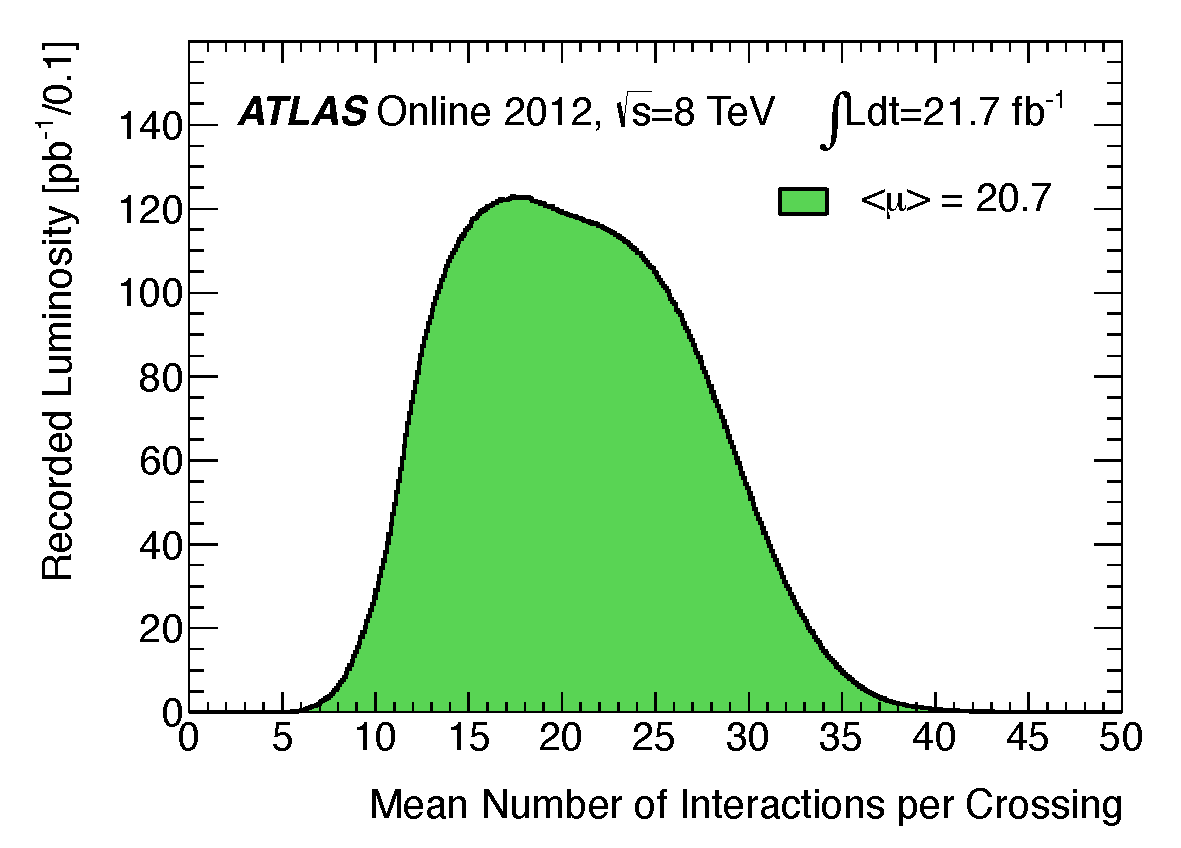
\includegraphics[width=0.8\textwidth]{/Users/caitlinmalone/Documents/Thesis/ReconstructionPerformance/images/mu_2012-dec.pdf}
	\label{fig:inner_detector}  
	\caption{}
\end{figure}

% http://cds.cern.ch/record/1435196/files/ATLAS-CONF-2012-042.pdf
\section{Track Reconstruction}
\label{sec:trk_reco}
%https://twiki.cern.ch/twiki/pub/AtlasPublic/EventDisplayStandAlone/2012_highPileup.png
Track reconstruction takes place in the inner detector and allows crucial measurements such as the primary and secondary vertices.  When a charged particle traverses the layers of the inner detector, it leaves typically 8-11 hits in silicon (counting one double-sided layer of SCT silicon as capable of seeing 2 hits) and about 35 in the TRT.  The track reconstruction algorithm, as detailed in section \ref{sec:trt}

Good identification of primary vertices is critical for disambiguating which collision a given particle comes from; with 20-40 collisions per bunch crossing in 2012, primary vertex resolution is nontrivial.  

% http://www.slac.stanford.edu/cgi-wrap/getdoc/slac-pub-5671.pdf
% http://www.quantumdiaries.org/2011/06/10/to-b-or-not-to-bbar-b-tagging-via-track-counting/
% http://dorigo.wordpress.com/2007/05/15/b-hadron-lifetimes-part-2/
\section{B-Tagging}




